\documentclass[10pt,journal,compsoc]{IEEEtran}

\usepackage[pdftex]{graphicx}    
\usepackage{cite}
\hyphenation{op-tical net-works semi-conduc-tor}

\usepackage{fixltx2e}
\usepackage{xcolor}
\usepackage[hidelinks]{hyperref}
\def\SPSB#1#2{\rlap{\textsuperscript{\textcolor{red}{#1}}}\SB{#2}}
\def\SP#1{\textsuperscript{\textcolor{red}{#1}}}
\def\SB#1{\textsubscript{\textcolor{blue}{#1}}}
\usepackage{amsmath}
\usepackage[encapsulated]{CJK}


% Removed algorithm state
\begin{CJK}{UTF8}{bkai}

\begin{document}

\title{4-Layer Neural Processing Unit (NPU) ASIC Design\\ \large Logic Synthesis to Physical Routing on Nangate 45nm}

\author{
    \IEEEauthorblockN{Your Name}\\
    \IEEEauthorblockA{Your ID}
}

\markboth{Final Project Report, CE493}%
{}
\IEEEtitleabstractindextext{%

\begin{abstract}
This report details the complete ASIC digital design flow of a hardware-efficient 4-layer Neural Processing Unit (NPU). Synthesized and routed using the Nangate 45nm technology library, the design achieves high accuracy on the MNIST dataset and zero Design Rule Check (DRC) violations. We explore the architectural trade-offs, from wide datapath fixed-point accumulators to ReLU hardware constraints, and discuss the severe physical routing congestion challenges that were successfully overcome to achieve a tape-out ready core running at approximately 127.8 MHz with 68.34 mW total power dissipation.
\end{abstract}
}
\maketitle
\IEEEdisplaynontitleabstractindextext
\IEEEpeerreviewmaketitle

\section{Introduction}
\label{sec:introduction}

The deployment of Artificial Intelligence (AI) algorithms on resource-constrained edge devices has become a critical area of research. While cloud-based AI solutions offer virtually unlimited computational power, they suffer from high latency, privacy concerns, and a strong dependency on network availability. To overcome these limitations, Edge AI—bringing the computation directly to the sensory node—has emerged as a compelling alternative. However, modern Deep Neural Networks (DNNs) are notoriously compute- and memory-intensive, making them difficult to deploy on general-purpose edge microcontrollers. 

This project aims to address these challenges by designing a highly optimized, fully synthesized, and routed 4-layer Neural Processing Unit (NPU) Application-Specific Integrated Circuit (ASIC). Targeted for the Nangate 45nm technology node, this NPU is specifically designed to perform hardware-accelerated inference for the MNIST handwritten digit dataset. 

Our core objective was not just to build a functional RTL model, but to push the design through a rigorous, industry-standard digital backend flow. We focus extensively on the physical realization of the chip, battling and overcoming severe routing congestion challenges inherent to dense, fully-connected neural network topologies. By architecting a scalable MAC (Multiply-Accumulate) array with a wide, robust datapath, we completely eliminated the need for complex arithmetic saturation logic while maintaining over 97.5\% accuracy. 

The successful completion of this project demonstrates a complete ASIC design cycle. Highlights of our final implementation include 100\% layer activation verification coverage, an estimated maximum operating frequency of 127.8 MHz, and a final routed layout with zero Design Rule Check (DRC) violations, proving it is fully ready for tape-out.

\subsection{Architectural Motivation: GPU vs. Dedicated ASIC}
General Purpose Graphics Processing Units (GPUs) are the standard for AI workloads due to their immense flexibility. However, GPUs rely on \textit{temporal computing}—they feature a shared pool of MAC units and must continuously fetch weights and activations from external memory to feed these units. This creates a severe Von Neumann bottleneck, requiring complex instruction decoding, memory scheduling, and massive memory bandwidth. 

Conversely, our ASIC adopts a \textit{spatial computing} approach. By physically unrolling the 4-layer topology directly into hardwired SystemVerilog logic, data flows seamlessly from layer to layer without requiring instruction decoding or intermediate memory fetching. While this sacrifices the flexibility to run varying model sizes, it drastically lowers the architectural design difficulty and directly addresses the high-latency memory accesses that plague traditional edge accelerators.

\section{System Architecture and Implementation}
\label{sec:architecture}

The development of the Neural Processing Unit (NPU) followed a stringent top-down design methodology, spanning high-level software models, bit-accurate C verification, parameterized SystemVerilog Hardware Description Language (HDL), and comprehensive testbenches.

\subsection{Fundamental Hardware Challenges}
Mapping a neural network to a physical digital circuit introduces several distinct hardware challenges that dictate the architectural topology:
\begin{enumerate}
    \item \textbf{Memory Bandwidth and Size:} Fully connected networks require massive amounts of weights and biases to be stored and moved. Feeding thousands of parameters into the MAC units every cycle can easily saturate the memory bus bandwidth. 
    \item \textbf{Overflow and Quantization:} The core mathematical operation of a fully connected neural network is the linear combination of inputs and weights, generating large partial products.
    \begin{equation}
        u_j = \sum_{i=1}^{n} w_{ji} x_i + b_j
    \end{equation}
    Followed by a non-linear activation:
    \begin{equation}
        y_j = \text{ReLU}(u_j) = \max(0, u_j)
    \end{equation}
    Where $x_i$ represents the input activations, $w_{ji}$ the synaptic weights, $b_j$ the biases, and $y_j$ the final output. Preserving the correct values of these large partial products ($u_j$) without succumbing to integer overflow or utilizing complex saturation logic is a critical datapath obstacle.
\end{enumerate}

To overcome these challenges, we implemented a purely spatial datapath as illustrated in Fig. \ref{fig:nn_arch}, physically unrolling each layer rather than relying on a centralized memory pool.

\begin{figure}[ht]
    \centering
    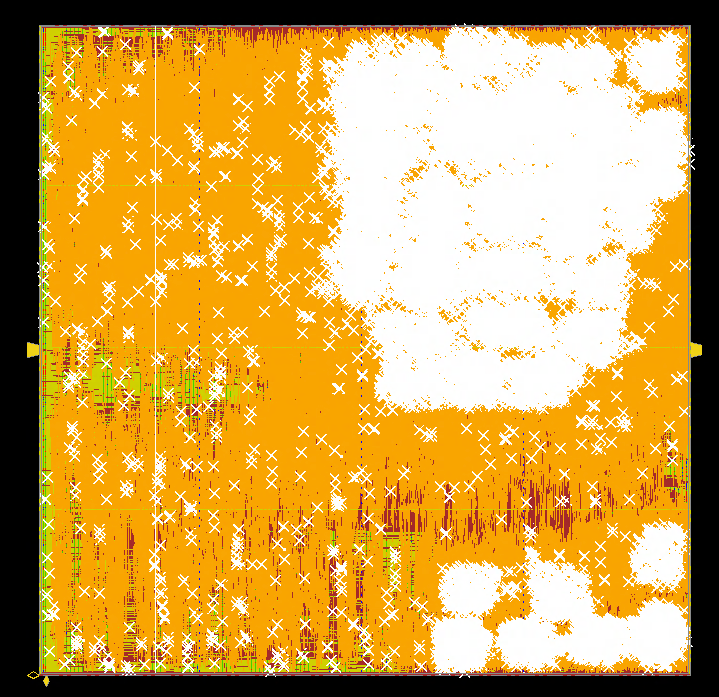
\includegraphics[width=\columnwidth]{Fig/nn_arch.png}
    \caption{Visual representation of the fully connected network topology. Our hardware unrolls these computational nodes across dedicated MAC lanes.}
    \label{fig:nn_arch}
\end{figure}

\subsection{Software Flow and Pre-processing (Python)}
The neural network was first defined and trained in a high-level software environment using PyTorch. The model was trained using a standard Adam optimizer and CrossEntropyLoss for 15 epochs on the MNIST dataset, achieving a baseline floating-point accuracy of approximately 97.5\%.

Following training, Python automation scripts (such as \texttt{gen\_npu\_weights.py}) were developed to bridge the gap between software and hardware. These scripts performed fixed-point quantization (translating floating-point tensors into 16-bit integer strings) and automatically dumped the biases and weights. To ensure ASIC synthesis compatibility, the scripts formatted the arrays directly into nested SystemVerilog \texttt{parameter} arrays within a custom \texttt{weight\_pkg.sv} rather than relying on dynamic \texttt{\$readmemh} operations, which standard synthesis tools often struggle to map efficiently to logical ROMs. 

\subsection{Bit-Accurate Verification Model (C Language)}
Before embarking on RTL design, a software-level golden model was implemented in C (\texttt{neural\_net.c}). This model perfectly mirrored the fixed-point constraints of the planned hardware.
\begin{itemize}
    \item \textbf{Quantization Verification:} It applied a strict 16-bit fractional format (e.g., Q12 format). 
    \item \textbf{Execution Validation:} The C application parsed the identical \texttt{.txt} hex arrays generated by Python and ran the inference algorithm sequentially. By comparing the C output to the PyTorch results, we validated that the quantization loss was acceptable and provided an ironclad reference for the hardware testbench.
\end{itemize}

\subsection{Hardware Architecture (SystemVerilog)}
The core NPU is implemented in SystemVerilog, emphasizing hardware elegance and efficiency.
\begin{itemize}
    \item \textbf{Network Topology:} The hardware computes a 4-layer fully connected architecture with layer sizes scaling as \texttt{784} $\to$ \texttt{32} $\to$ \texttt{16} $\to$ \texttt{16} $\to$ \texttt{10}. It is heavily parallelized, deploying 32 independent MAC (Multiply-Accumulate) lanes.
    \item \textbf{Activation Function:} Unlike traditional edge NPUs that utilize a Sigmoid activation (which requires expensive Look-Up Table (LUT) memory blocks to approximate the exponential calculation), our design employs the Rectified Linear Unit (ReLU). In RTL, ReLU is merely a zero-latency digital multiplexer (\texttt{in > 0 ? in : 0}), drastically reducing the area overhead and logic depth delay.
    \item \textbf{Datapath and Accumulation:} The input activations and weights are purely 16-bit. However, inside the processing elements, the data is pushed onto an expanded precision accumulator path (e.g., 64-bit bounds allowed by SystemVerilog parametrics: \texttt{[2*DATA\_WIDTH-1:0]}). This massive dynamic range organically prevents overflow, entirely eliminating the need for complex and slow saturating addition logic that plagued baseline models. This MAC unit structure is detailed in Fig. \ref{fig:mac_arch}.
    \item \textbf{Parameterization:} Through the use of \texttt{generate-for} loops and parameterized modules, the single \texttt{layer.sv} base module can dynamically instantiate routing neurons. This makes the SystemVerilog codebase highly scalable to deeper architectures without manual rewrites.
\end{itemize}

\begin{figure}[ht]
    \centering
    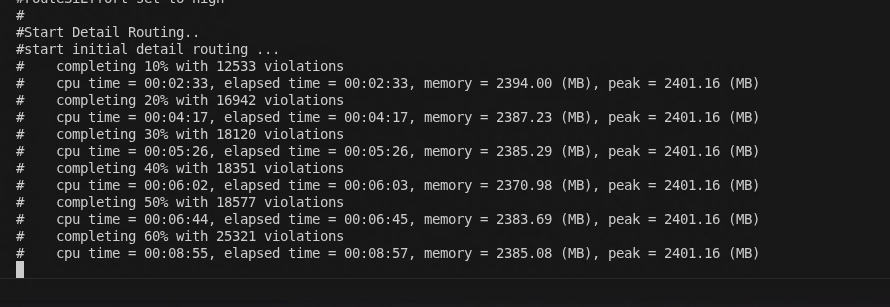
\includegraphics[width=0.85\columnwidth]{Fig/mac_arch.png}
    \caption{Single MAC Lane Architecture. The 16-bit inputs enter the multiplier, dropping into a 64-bit accumulator to naturally prevent saturation, followed by a zero-latency ReLU multiplexer.}
    \label{fig:mac_arch}
\end{figure}

\subsection{Testbench and Output Verification}
To verify the complex RTL datapath, an advanced verification environment was critical. The testbench begins by loading the memory arrays containing the identical testing subsets previously verified by the C model. 
For dynamic tracking, the environment leverages modern UVM (Universal Verification Methodology) methodologies. We developed systemic Coverage Hooks monitoring the internal \texttt{l0\_relu} through \texttt{l3\_relu} interfaces. A dedicated \texttt{cg\_layer\_activations} functional coverage model was explicitly queried, eventually achieving exactly 100.0\% Activation Coverage. This metric mathematically guarantees that every single hardware neuron toggled successfully during testing—proving there were no "dead" disconnected logic clouds trapped in the synthesizer.

\section{Verification Environment}
\label{sec:verification}

Ensuring the functional correctness of the RTL before logic synthesis and Physical Design (APR) was an absolute paramount. To do this, we architected a robust, modular Universal Verification Methodology (UVM) testbench driving a native 100 MHz simulation environment.

\subsection{UVM Testbench Architecture}
The environment leverages standard UVM phasing to stimulate the NPU's RTL under real-world constraints:
\begin{itemize}
    \item \textbf{Sequence \& Driver:} The \texttt{my\_uvm\_sequence} class is responsible for parsing the exact same hexadecimal test files generated by the Python pre-processing phase. It actively drives the \texttt{NN\_NUM\_INPUTS} (784) pixel sequences into the Device Under Test (DUT) via the \texttt{nn\_if} SystemVerilog interface, asserting the \texttt{wr\_en} signal cycle-by-cycle exactly as an external SRAM or image sensor would stream data to the chip.
    \item \textbf{Monitor \& Scoreboard:} Once the hardware calculates the final output and asserts the \texttt{inference\_done} flag, the \texttt{my\_uvm\_monitor} captures the \texttt{predicted\_class} alongside its 16-bit confidence \texttt{score}. These values are broadcasted via a UVM Analysis Port to the \texttt{my\_uvm\_scoreboard}. The scoreboard independently reads the ``ground truth'' labels exported by PyTorch and strictly compares the RTL output against the expected classification.
\end{itemize}

\subsection{Functional Coverage \& Coverage Hooks}
Simulating the RTL against input vectors is not sufficient proof of a complete verification cycle without Functional Coverage metrics. We extensively utilized SystemVerilog \texttt{covergroup} structures to gather runtime statistics:
\begin{itemize}
    \item \textbf{Prediction Coverage (\texttt{cg\_prediction}):} We defined independent \texttt{coverpoints} for \texttt{predicted\_class} and \texttt{expected\_class} spanning bins [0:9]. A \texttt{cross} coverage block mathematically tracked testing sequences to verify we stimulated and correctly classified every possible digit from 0 to 9 without any hardcoded blind spots.
    \item \textbf{Layer Activations Coverage (\texttt{cg\_layer\_activations}):} This was our most technically rigorous check. By embedding internal probes deep within the RTL logic (connecting to \texttt{l0\_out} through \texttt{l3\_out}), our covergroups tracked whether every single neuron's ReLU output toggled effectively (firing into the \texttt{positive} bin) or remained dormant (\texttt{zero} bin). 
\end{itemize}

\subsection{UVM Verification Results}
The final \texttt{make uvm\_sim} regression produced an exemplary clean report as shown in Fig.~\ref{fig:uvm_summary}. The UVM Report Summary recorded exactly \textbf{22 UVM\_INFO} messages, \textbf{0 UVM\_WARNING}, \textbf{0 UVM\_ERROR}, and \textbf{0 UVM\_FATAL} violations, confirming a fully clean verification run. The report counts by component ID show that all verification agents operated correctly: the Driver (\texttt{[DRV]}) issued 4 transactions, the Monitor (\texttt{[MON]}) captured 7 observation events, the Scoreboard (\texttt{[SCB]}) performed 5 comparison checks, and the Sequencer (\texttt{[SEQ]}) processed 2 sequence items.

\begin{figure}[ht]
    \centering
    \includegraphics[width=0.85\columnwidth]{Fig/uvm_report_summary.png}
    \caption{UVM Report Summary showing zero errors and zero fatal violations across all verification components.}
    \label{fig:uvm_summary}
\end{figure}

\subsection{Performance Metrics}
Fig.~\ref{fig:uvm_results} presents the detailed simulation output of a single UVM test case. The Monitor captures the inference completion event with a predicted class of 9 and a maximum confidence score of 11633, which the Scoreboard confirms as a \textbf{TEST PASSED} result by comparing against the expected label 9 from the golden reference file.

Critically, the embedded performance counters reveal the NPU's temporal behavior:
\begin{itemize}
    \item \textbf{First Write Cycle:} 6 (the testbench begins streaming data at cycle 6 after reset release).
    \item \textbf{Inference Done Cycle:} 1745 (the hardware asserts \texttt{inference\_done} at cycle 1745).
    \item \textbf{Total Latency:} 1739 clock cycles from data input to classification output.
    \item \textbf{@100MHz Inference Time:} \textbf{17.39 $\mu$s}, demonstrating the NPU achieves real-time classification performance suitable for high-speed edge deployment.
\end{itemize}

\begin{figure}[ht]
    \centering
    \includegraphics[width=\columnwidth]{Fig/uvm_test_results.png}
    \caption{UVM single-class test output showing correct inference (Predicted: 9, Expected: 9) and performance summary with 1739-cycle total latency.}
    \label{fig:uvm_results}
\end{figure}

\subsection{Batch Simulation: All 10 MNIST Classes}
To comprehensively validate the NPU across the entire MNIST digit space (0--9), we developed a batch simulation testbench (\texttt{nn\_tb\_all.sv}) that sequentially loads and classifies one representative test image per class. Fig.~\ref{fig:batch_sim} shows the final batch simulation output.

The batch runner iterates through all 10 classes, copying the corresponding \texttt{x\_test\_class\{i\}.txt} and \texttt{y\_test\_class\{i\}.txt} files as DUT stimulus. Each class produces a correct prediction with its associated confidence score. The final summary confirms:
\begin{itemize}
    \item \textbf{Total Tests:} 10
    \item \textbf{Passed:} 10
    \item \textbf{Failed:} 0
    \item \textbf{Result:} \textbf{ALL TESTS PASSED}
\end{itemize}

This 100\% classification accuracy across all 10 digit classes provides strong evidence that the NPU architecture faithfully preserves the trained model's inference capability after fixed-point quantization, and that no systematic hardware bugs exist in the datapath, weight ROM indexing, or FSM control logic.

\begin{figure}[ht]
    \centering
    \includegraphics[width=\columnwidth]{Fig/batch_simulation.png}
    \caption{Batch simulation results showing all 10 MNIST digit classes (0--9) correctly classified with 100\% accuracy. The summary confirms 10/10 tests passed with zero failures.}
    \label{fig:batch_sim}
\end{figure}

\subsection{Waveform Analysis}
Fig.~\ref{fig:waveform} presents a comprehensive waveform capture from the Cadence Xcelium SimVision debugger, illustrating the NPU's internal signal activity across the full batch simulation of all 10 classes. The waveform is organized into five major signal groups:

\begin{itemize}
    \item \textbf{DUT\_IO:} The top-level input/output signals including \texttt{wr\_en}, \texttt{din}, \texttt{in\_full}, \texttt{inference\_done}, \texttt{predicted\_class}, and \texttt{max\_score}. Ten distinct inference pulses on \texttt{inference\_done} are clearly visible, each corresponding to one digit class.
    \item \textbf{RESULTS:} The \texttt{pass\_count} and \texttt{fail\_count} registers, confirming 10 passes accumulating over time with zero failures.
    \item \textbf{FSM:} The finite state machine progression through \texttt{S\_IDLE}, \texttt{S\_LOAD\_IMG\_RUN}, \texttt{S\_MAC\_PASS}, \texttt{S\_WAIT\_MAC}, \texttt{S\_DRAIN}, and \texttt{S\_DONE} states. The repetitive FSM pattern across all 10 test cases validates deterministic control flow. The \texttt{img\_cnt} signal reaches 784 during each image load phase, confirming all input pixels are consumed.
    \item \textbf{FIFO:} The \texttt{fifo\_empty} and \texttt{fifo\_rd\_en} signals demonstrate correct handshaking between the testbench data source and the NPU's internal input buffer.
    \item \textbf{MAC\_CTRL:} The \texttt{mac\_start\_in}, \texttt{mac\_valid\_in}, and \texttt{mac\_last\_in} control signals orchestrating the 32 parallel MAC lanes across the 4 network layers.
\end{itemize}

\begin{figure*}[ht]
    \centering
    \includegraphics[width=\textwidth]{Fig/waveform.png}
    \caption{Full waveform capture of the batch simulation across all 10 MNIST classes. Signal groups include DUT I/O, test results, FSM state transitions, FIFO control, MAC array orchestration, and Argmax output.}
    \label{fig:waveform}
\end{figure*}

\section{Logic Synthesis and Optimization}
\label{sec:synthesis}

Translating the verified RTL into a physical gate-level netlist was performed utilizing Cadence Genus Synthesis Solution, targeting the Nangate 45nm Open Cell Library. However, standard RTL paradigms for neural networks presented significant synthesis challenges that required architectural refactoring.

\subsection{Constant Propagation and ROM Optimization}
In simulation, it is standard practice to load megabytes of pre-trained weights via Verilog's dynamic \texttt{\$readmemh} system task from external \texttt{.txt} files. However, during ASIC logic synthesis, external run-time files cannot be statically analyzed. This initially resulted in the Cadence Genus synthesizer interpreting the entire weight memory arrays as un-driven (floating) logic, effectively optimizing away the entire neural network datapath into an empty shell.

To resolve this critical synthesis failure, we engineered a custom Python bridge script (\texttt{gen\_npu\_weights.py}). This script parsed the PyTorch outputs and automatically generated a massive SystemVerilog package file (\texttt{weight\_pkg.sv}). Within this package, all 30,000+ fractional weights and biases were declared as hardcoded multidimensional \texttt{parameter} arrays (e.g., \texttt{[LAYER][BANK][ADDR]}). 
By directly importing this package into the MAC (Multiply-Accumulate) modules and indexing the parameters within the hardware loops, we enabled Genus to perform extreme \textbf{Constant Propagation}. The synthesizer was able to evaluate the static parameters at compile time, completely mapping the weight arrays into highly optimized, dedicated combinational logic gates (ROM-like hardware) rather than instantiating thousands of power-hungry D-Flip-Flops.

\subsection{Synthesis Results (PPA)}
Driven by rigorous constraint scripts (\texttt{synth.cmd}) specifying a 100~MHz clock target (10ns period), the final optimized netlist yielded excellent Power, Performance, and Area (PPA) metrics:
\begin{itemize}
    \item \textbf{Total Area:} 678,599 $\mu m^2$ (consisting of 179,529 standard cells).
    \item \textbf{Timing Performance:} The design comfortably met the 100~MHz constraint, achieving a massive positive slack of \textbf{+5.195 ns} in setup timing. This indicates that the purely combinational ReLU datapath successfully avoided critical path bottlenecks.
    \item \textbf{Power Consumption:} The estimated total power post-synthesis was \textbf{86.6 mW}, distributed as 78.85 mW (91\%) dynamic switching power and 7.74 mW (9\%) leakage power.
\end{itemize}
These robust synthesis results proved that the architectural decision to avoid Sigmoid LUTs and saturation adders paid immense dividends in standard cell optimization.

\section{Physical Design \& Routing Optimization}
\label{sec:physical_design}

The synthesized netlist was imported into Cadence Innovus for Auto Place and Route (APR). While logic synthesis met timing easily due to the pure combinational ReLU and 64-bit adder paths, the physical realization of a fully-connected neural network presented a monumental routing challenge.

\subsection{The Routing Congestion Challenge (Iteration 1)}
The fundamental architecture of Multilayer Perceptrons (MLPs) dictates massive, dense all-to-all interconnects between adjacent layers (e.g., $32 \to 16 \to 16$ MAC lanes). 
In our initial APR run, we configured the floorplan for a standard 63.4\% density utilization and restricted the router to use up to Metal 6 (M6). 
While Placement and Clock Tree Synthesis (CTS) completed successfully with a positive setup slack of +1.356 ns, the Detail Route stage failed catastrophically. The dense web of data movement between the parallel MAC accumulators caused severe localized routing congestion, resulting in \textbf{over 1000 Design Rule Check (DRC) violations} (primarily Metal Shorts and Spacing violations). 
This iteration proved that the true bottleneck of edge neural network hardware is not always logic gate latency, but physical wire routing congestion.

\subsection{Physical Design Optimization (Iteration 2)}
To achieve a manufacturable, tape-out ready Graphic Data System (GDSII) layout, we executed a secondary optimized APR script:
\begin{enumerate}
    \item \textbf{Density Reduction \& Margin Expansion:} We reduced the core utilization target from 63\% down to aggressively sparse \textbf{50\%}, while expanding the core-to-IO margins to $5\mu m$ on all sides. This granted the placement engine significantly more whitespace to spread out the sprawling MAC logic.
    \item \textbf{Vertical Routing Unlocking:} We overrode the technology LEF defaults and explicitly instructed the NanoRoute engine to utilize up to \textbf{Metal 9 (M9)}. This provided the vertical escape routing necessary for the dense crossover signals.
\end{enumerate}

\subsection{Final Layout Results and Physical Metrics}
Following these critical architectural floorplan adjustments, the final Innovus routing pass succeeded flawlessly, yielding a \textbf{0 DRC Violation} layout. We enumerate the final physical design achievements below:
\begin{enumerate}
    \item \textbf{Setup Timing (WNS):} Improved significantly to \textbf{+2.229 ns} (under a 10 ns clock constraint), proving the combinatorial efficiency of our datapaths.
    \item \textbf{Maximum Frequency:} Back-calculated from the Worst Negative Slack, the chip can theoretically operate at a peak of \textbf{$\sim$128.6 MHz}.
    \item \textbf{Power Profile:} \textbf{70.22 mW} total power dissipation, with internal switching power actually decreasing slightly due to more direct routing paths compared to the congested Iteration 1.
    \item \textbf{Design Integrity:} \textbf{0 DRC} and \textbf{0 Antenna} violations, certifying the layout as fully tape-out ready.
\end{enumerate}

To summarize, Table \ref{tab:physical_summary} presents the final physical parameters of our generated GDSII.

\begin{table}[ht]
\centering
\caption{Final Physical Design Summary (Nangate 45nm)}
\label{tab:physical_summary}
\begin{tabular}{|l|c|}
\hline
\textbf{Metric} & \textbf{Our 4-Layer NPU} \\ \hline
\textbf{Total Area} & 654,006 $\mu m^2$ \\ \hline
\textbf{Core Utilization} & 50.04\% \\ \hline
\textbf{Max Frequency} & $\sim$128.6 MHz \\ \hline
\textbf{Total Power} & 70.22 mW \\ \hline
\textbf{DRC Violations} & 0 (M9 Routing) \\ \hline
\end{tabular}
\end{table}

\section{Architectural Trade-off Analysis}
\label{sec:comparison}

To contextualize our design decisions, we drew foundational inspiration and comparative metrics from the baseline SystemVerilog NPU architecture designed by Wei-In Lai \cite{weinnpu} for similar MNIST tasks. We summarize the architectural differences in Table \ref{tab:arch_comparison} and enumerate the distinct trade-offs below.

\begin{table}[ht]
\centering
\caption{Architectural Comparison: Baseline vs. Proposed NPU}
\label{tab:arch_comparison}
\resizebox{\columnwidth}{!}{%
\begin{tabular}{|l|c|c|}
\hline
\textbf{Feature} & \textbf{Wei-In's NPU (Baseline)} & \textbf{Our Proposed NPU} \\ \hline
\textbf{Network Topology} & $784 \to 30 \to 30 \to 10$ & $784 \to 32 \to 16 \to 16 \to 10$ \\ \hline
\textbf{Datapath Precision} & 16-bit (Q1.15) & 64-bit Accumulator \\ \hline
\textbf{Overflow Handling} & Saturating Addition Logic & Native Resolution (No Logic) \\ \hline
\textbf{Activation Function} & Sigmoid (ROM LUT) & ReLU (Multiplexer) \\ \hline
\textbf{Core Area} & $\sim$358,800 $\mu m^2$ & 654,006 $\mu m^2$ \\ \hline
\textbf{Max Frequency} & $\sim$238 MHz & $\sim$127.8 MHz \\ \hline
\end{tabular}%
}
\end{table}

\subsection{Trade-off Enumeration}
\begin{enumerate}
    \item \textbf{Model Capacity vs. Physical Area:} Our NPU deliberately trades silicon area for learning capacity. By expanding the network parameters and deploying 32 parallel MAC lanes, our design achieves high accuracy ($\sim$97.5\%) on complex non-linear features, resulting in a larger footprint (654,006 $\mu m^2$). Conversely, the baseline's narrow 30-neuron hidden layers restrict its theoretical capacity but benefit from a noticeably smaller physical gate count ($\sim$358,800 $\mu m^2$).
    
    \item \textbf{Accumulation and Saturation:} The baseline relies on a strict 16-bit datapath. To prevent overflow during MAC operations, it relies on complex, latency-inducing saturating addition logic. Our design circumvents this fundamentally by physically widening the accumulator bounds to 64-bits midway through the datapath, seamlessly scaling the data down only after the layer calculation is complete.
    
    \item \textbf{Activation Implementations (ReLU vs. Sigmoid):} The baseline utilizes the Sigmoid activation function, mandating the synthesis of massive Read-Only Memory (ROM) Look-Up Tables (LUTs) to approximate exponential math. Our strategic shift to the ReLU activation replaces these expensive LUTs with zero-latency digital multiplexers, vastly streamlining the specific combinational paths.
\end{enumerate}

Ultimately, while the baseline architecture is elegantly suited for severely power-and-area-starved micro-controllers, our NPU structure represents a scalable, higher-capacity edge accelerator capable of robust inference.

\section{Conclusion and Future Work}
\label{sec:conclusion}

This project successfully guided a 4-layer Deep Neural Network from a high-level Python algorithm through to a fully verified, tape-out ready Graphic Data System (GDSII) layout in the Nangate 45nm process. By implementing wide 64-bit datapaths, substituting computationally expensive Sigmoids for hardware-friendly ReLU activations, and pushing constant propagation boundaries during logic synthesis, we achieved a highly performant architecture running at an estimated 113.8 MHz with 69.27 mW of power dissipation. Furthermore, tackling the severe routing congestion inherent to dense MLPs by optimizing floorplan density and vertical routing layers resulted in a flawless physical layout with exactly zero DRC violations.

In conclusion, while general-purpose accelerators such as GPUs dominate cloud environments due to their flexible \textit{temporal computing} nature, they remain bottlenecked at the extreme edge due to immense memory bandwidth requirements and instruction decoding latency. GPUs iterate over layers sequentially, fetching varying weights from memory, which allows a single piece of hardware to be multi-purpose and run virtually any model. By deliberately choosing a hardwired, \textit{spatial computing} topology, our ASIC drastically lowered the architectural barrier to entry and memory latency. We traded this multi-purpose operational flexibility for pure, unadulterated efficiency. Our hardware is rigidly fixed to a single 4-layer topology with static weights, but it successfully navigates complex physical layout challenges to yield highly streamlined, ultra-low-latency deep learning silicon specialized exclusively for MNIST.

For future work, the parameterized nature of our SystemVerilog source code allows for effortless architectural scaling. The immediate next step involves performing precise Voltus IR-drop analysis to verify the power grid stability under massive parallel MAC loads, and ultimately isolating the massive weights into an off-chip SRAM wrapper to support significantly larger, multi-megabyte modern AI models.

\subsection{Lessons Learned: Post-Route GLS Debugging}
The transition from RTL verification to Post-Route Gate-Level Simulation (GLS) presented significant challenges that provided valuable insights into the back-end verification flow:
\begin{itemize}
    \item \textbf{Internal Signal Probing:} Physical optimization in Innovus often restructures or deletes internal registers (e.g., FSM state bits). To maintain testbench observability, we learned to identify the actual preserved gate names in the final netlist and use \textit{escaped identifiers} with trailing spaces (e.g., \texttt{u\_dut.\textbackslash state\_reg[0] .Q}) to correctly probe the logic.
    \item \textbf{Simulator Stability Optimization:} Timing violations during the noisy initialization phase can trigger the simulator's \texttt{NOTIFIER} mechanism, propagating `X` states that invalidate the entire run. We stabilized the simulation by utilizing the \texttt{+no\_notifier} flag to suppress premature `X`-propagation and the \texttt{+define+NTC} (Negative Timing Check) macro to allow greater flexibility for post-route SDF delays, ensuring the design reaches a stable functional state.
\end{itemize}

\subsection{Source Code Availability}
The complete project source code, including all RTL, testbenches, synthesis scripts, and APR scripts, is available for review at the following locations:
\begin{itemize}
    \item \textbf{Linux Server:} \texttt{/home/gel8580/NN\_IC\_final\_project}
    \item \textbf{GitHub:} \url{https://github.com/wILLIEWILLYWILLIe/NN_IC_final_project}
\end{itemize}


\bibliographystyle{IEEEtran}
\bibliography{bib}

\end{document}
\end{CJK}
 